\documentclass[../tesis_main.text]{subfiles}

\chapter{Manipulador}
	En esta sección se hablará de las caracteriscias mecánicas del brazo robótico ensamblado en el robot de servicio Justina. Se describirán los elementos que componen el brazo robótico haciendo enfasís en la ubicación de los actuadores y como influye esto en el modelo matematico del mismo.


%%%%%%%%%%%%%%%%%%%%%%%%%%%%%%%%%%%%%%%%%%%%%%%%%%%%%%%%%%%%%%%%
           %%%%%%  DESCRPCIÓN SERVOMOTORES   %%%%%%%%
%%%%%%%%%%%%%%%%%%%%%%%%%%%%%%%%%%%%%%%%%%%%%%%%%%%%%%%%%%%%%%%%
	\section{Documentación servos dynamixel}
		Los servomotores Dynamixel son un sistema de actuador inteligente desarrollados con el propósito de funcionar como uniones de conexión en un robot o estructura mecánica. Los servomotores Dynamixel están diseñados para ser modulares y soportar la conexión en cadena en cualquier robot o diseño mecánico. Este tipo de servomotores es popular por los beneficios que ofrece: movimientos robóticos potentes y flexibles.\\

		El conjunto de servomotores Dynamixel son un grupo de actuadores de alto rendimiento con reductor, controlador y un protocolo de red completamente integrados en un módulo de servomotor programable y en red. El estado del actuador se puede leer y monitorear a través de un flujo de paquetes de datos. \cite{dynamixelEpage}\\

		Los servomotores de la marca Dynamixel, cuentan con diferentes gamas de productos de acuerdo a las necesidades de cada proyecto. El brazo robótico referente a este documento está constituido unicamente por motores de la gama MX, de la cual se describen las caracteristicas más sobresalientes a continuación.\\  

			\subsection{Motores dynamixel Serie MX}
		Los actuadores dynamixel de la serie MX pertencen a la última generación de actuadores de la companñia Robotis Dynamixel. Están equipados con un procesador Cortex M3 de 32 bits a 72 mhz, un encoder magnético sin contacto con una resolución 4 veces mayor que la serie AX / RX, además ofrecen una velocidad de comunicación de hasta 3 mbps con el nuevo bus TTL 2.0. Cada servomotor cuenta con la capacidad  de monitorear su velocidad, temperatura, posición del eje, voltaje y carga.\\

		Por otro lado los motores Dynamixel de la seire MX cuentan con la implemntación de un algoritmo de control PID para mantener la posición del eje. Las ganancias del algoritmo de control PID se pueden ajustar individualmente para cada servo, lo que le permite controlar la velocidad y la fuerza de la respuesta del motor. Todos los servos de la serie MX usan un voltaje nominal de 12v. La característica más importante de esta seie de servomotores es que la gestión de la información proveniente del sensor y la ejecución del algoritmo de control de posición son manejados por el microcontrolador integrado del servo. Este enfoque distribuido deja a su controlador principal libre para realizar otras funciones.\\


		En lo que respecta a la parte mecánica, todos los servos DYNAMIXEL son compatibles con una amplia variedad de bridas, acoplamientos y sujetadores lo cual facilita la construcción de cualquier configuración deseada. Este conjunto de elementos mecánicos permite una conección directa cualquier modelo de servomotores DYNAMIXEL, lo que le permite una gran variedad de configuraciones para cualquier necesidad. Dada la gran variedad de configuraciones, este tipo de elementos de unión y fijación resultó de gran ayuda mecánica al momento de contruir el brazo robótico donde se implentaron los algoritmos descritos en el presente trabajo.\\

		\begin{figure}[h!]
			\begin{center}
			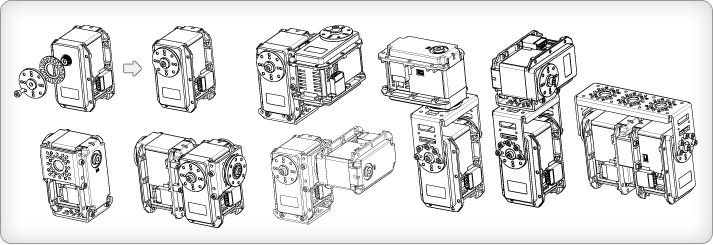
\includegraphics[width=14.5cm, height=6.5cm]{/dynamixel_conexions.jpg}	
			\caption{Variedad de ensambles para servomotores.}
			\end{center}
		\end{figure}

		Resuminedo las características de los sermovomotores de la serie MX, podemos enlistar las siguientes:\\ 

		\begin{itemize}
			\item{Movimiento sin contacto y detección de posición.}
			\item{Interfaz de comunicación TTL estándar.}
			\item{Comunicación de alta velocidad de hasta 4.5 Mbps.}
			\item{Control PID para autocorrección en posicionamiento.}
			\item{Control de par basado en corriente (4096 steps, 2.69mA/step)}
			\item{Ahorro de energía (corriente reducida de 100 mA a 40 mA)}
		\end{itemize}

		Si desea controlar este servo DYNAMIXEL desde un equipo de computo es necesario contar con un dispositivo que facilite la comunicación entre este y el microprocesador de cada uno de los servomotores, el dispositivo que cumple con esta funcionalidad es el USB2Dynamixel.\\

		El controlador USB2Dynamixel se conecta al puerto USB en una computadora y tiene un puerto de 3 y 4 pines para conectar Dynamixels. El USB2Dynamixel se puede usar con controladores como CM-5 y CM-2 que usan comunicación en serie, además soporta la comunicación en cadena propia de los servomotores Dynamixel. Es impornate mencionar que este dispositivo posee un interruptor para seleccionar entre diferentes protocolos de comunicación: RS-232, RS-485, TTL. Por tanto consta de:\\

		\begin{itemize}
			\item{Conector 3P: puerto de comunicación para nivel TTL (para control de serie AX y MX)}
			\item{Conector 4P: puerto de comunicación RS-485 (para control de serie DX, RX, EX y MX)}
		\end{itemize}


		\begin{figure}[h!]
			\begin{center}
			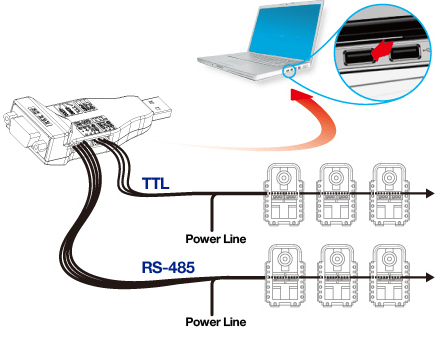
\includegraphics[width=10.5cm, height=8.5cm]{/usb2dynamixel.jpg}	
			\caption{Dispositivo de comunicación USB a protocolo serial.}
			\end{center}
		\end{figure}

		Los motores que componen esta gama comparten caracteristicas, las cuales se menacionan a continuación:\\

\begin{tabular}{ |p{6.5cm}||p{2.1cm}|p{2.1cm}|p{2.1cm}|  }
 \hline
 \multicolumn{4}{|c|}{\textbf{MOTORES GAMA MX} } \\
 \hline
 Voltaje de operación  &  14.8v   &	   12v   &   11.1v\\
 \hline
 Protocolo             &  \multicolumn{3}{|c|}{TTL Serial Asincrono} \\
 \hline
 Velocidad del puerto  &  \multicolumn{3}{|c|}{8000bps - 3Mbps} \\
 \hline
 Retroalimentación de posición & \multicolumn{3}{|c|}{ SI} \\
 \hline
 Retroalimentación de temperatura & \multicolumn{3}{|c|}{ SI}\\
 \hline
 Control PID           & \multicolumn{3}{|c|}{ SI } \\
 \hline
 Material              & \multicolumn{3}{|c|}{ Carcasa platica y reducción metálica} \\
 \hline
 Motor                 & \multicolumn{3}{|c|}{ Maxon RE-MAX} \\
 \hline
\end{tabular}\\

		Los modelos de motores que componen esta gama difieren en caracteríticas tales como las dimensiones, el par máximno a rotor bloqueado, la corriente máxima, o la velocidad máxima. A continuación se en listan las características más sobresalientes para cada modelo de motor.\\ 


		\subsection{Características MX-106}

\begin{tabular}{ |p{6.5cm}||p{2.1cm}|p{2.1cm}|p{2.1cm}|  }
 \hline
 \multicolumn{4}{|c|}{\textbf{MX-106} } \\
 \hline
 Voltaje de operación  &  14.8v   &	   12v   &   11.1v\\
 \hline
 Par de bloqueo        &  102kg.cm  &  85.6kg.cm  &  81.5kg.cm\\
 Velocidad sin carga   &  55rpm     &  45rpm      &  41rpm\\
 \hline
 Peso                  &  \multicolumn{3}{|c|}{153g} \\
 \hline
 Tamaño                &  \multicolumn{3}{|c|}{40.2 x 65.1 x 46 mm} \\
 \hline
 Resolución            &  \multicolumn{3}{|c|}{ 0.088 grado/valor de registro} \\
 \hline
 Relación de reducción &  \multicolumn{3}{|c|}{1/200} \\
 \hline
 Corriente máxima      &  \multicolumn{3}{|c|}{5.2A @ 12V} \\
 \hline
\end{tabular}

\begin{figure}[h!]
	\begin{center}
	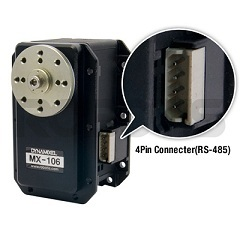
\includegraphics[width=8.5cm, height=8.5cm]{/MX_106R_2.jpg}	
	\caption{Servomotor dynamixel modelo MX-106.}
	\end{center}
\end{figure}


		\subsection{Características MX-64}

\begin{tabular}{ |p{6.5cm}||p{2.1cm}|p{2.1cm}|p{2.1cm}|  }
 \hline
 \multicolumn{4}{|c|}{\textbf{MX-64} } \\
 \hline
 Voltaje de operación  &  14.8v   &	   12v   &   11.1v\\
 \hline
 Par de bloqueo        &  74kg.cm   &  61kg.cm   &  56kg.cm\\
 Velocidad sin carga   &  78rpm     &  63rpm     &  58rpm\\
 \hline
 Peso                  &  \multicolumn{3}{|c|}{126g} \\
 \hline
 Tamaño                &  \multicolumn{3}{|c|}{40.2 x 61.1 x 41 mm} \\
 \hline
 Resolución            &  \multicolumn{3}{|c|}{ 0.088 grado/valor de registro} \\
 \hline
 Relación de reducción &  \multicolumn{3}{|c|}{1/200} \\
 \hline
 Corriente máxima      &  \multicolumn{3}{|c|}{4.1A @ 12V} \\
 \hline
\end{tabular}

\begin{figure}[h!]
	\begin{center}
	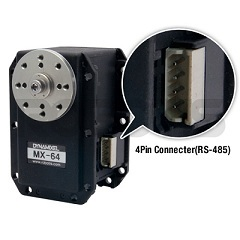
\includegraphics[width=8.5cm, height=8.5cm]{/MX_64R_2.jpg}	
	\caption{Servomotor dynamixel modelo MX-64.}
	\end{center}
\end{figure}

		\subsection{Características MX-28}

\begin{tabular}{ |p{6.5cm}||p{2.1cm}|p{2.1cm}|p{2.1cm}|  }
 \hline
 \multicolumn{4}{|c|}{\textbf{MX-28} } \\
 \hline
 Voltaje de operación  &  14.8v   &	   12v   &   11.1v\\
 \hline
 Par de bloqueo        &  31.6kg.cm  &  25.5kg.cm   &  23.4kg.cm\\
 Velocidad sin carga   &  67rpm      &  55rpm       &  50rpm\\
 \hline
 Peso                  &  \multicolumn{3}{|c|}{72g} \\
 \hline
 Tamaño                &  \multicolumn{3}{|c|}{35.6 x 50.6 x 35.5 mm} \\
 \hline
 Resolución            &  \multicolumn{3}{|c|}{ 0.088 grado/valor de registro} \\
 \hline
 Relación de reducción &  \multicolumn{3}{|c|}{1/193} \\
 \hline
 Corriente máxima      &  \multicolumn{3}{|c|}{1.4A @ 12V} \\
 \hline
\end{tabular}

\begin{figure}[h!]
	\begin{center}
	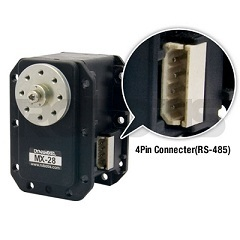
\includegraphics[width=8.5cm, height=8.5cm]{/MX_28R_2.jpg}	
	\caption{Servomotor dynamixel modelo MX-64.}
	\end{center}
\end{figure}

	Por otro lado es importante conocer la estructura de transmisión de la información de un servomotor con el dispositivo controlador. Para ello los servomotores dynamixel cuentan con un protocolo de comunicación serial asincrono, el cúal transtite una serie de datos en una trama, como se ilustra en la figura[].\\

	\begin{figure}[h!]
		\begin{center}
		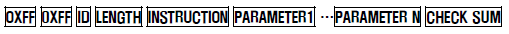
\includegraphics[width=15.5cm, height=1.5cm]{/trama.png}
		\end{center}
	\end{figure}

	El significado de cada byte que compone al paquete datos es el siguiente:\\

	\begin{itemize}
		\item{ \textbf{0xFF 0xFF} :  Es la instrucción que marca el inicio del paquete.}
		\item{ \textbf{ID} :  Es el ID de cada servomotor partícular en la cadena.}
		\item{ \textbf{LENGTH} :  Es el tamaño del paquete. El tamaño es calculado como el numero de parametros más dos (N+2).}
		\item{ \textbf{INSTRUCTION} :  Indica el tipo de instrucción que ejecutará el servomotor dynamixel.}
		\begin{itemize}
			\item{PING}
			\item{READ\_DATA}
			\item{WRITE\_DATA}
			\item{REG\_WRITE}
			\item{ACTION}
			\item{RESET}
			\item{SYN\_WRITE}
		\end{itemize}
		\item{ \textbf{PARANETER 0...N} :  Este parámetro se usa cuando la instrucción requiere datos auxiliares.}
		\item{ \textbf{CHECK SUM} :  Se usa para verificar si el paquete de datos se dañó durante la comunicación.}
	\end{itemize}
	
	A continuación se anexa una tabla con las caracteriticas más reelevantes de los registros que posee cada uno de los revomotores dynamixel.\\

\begin{tabular}{ |p{1.2cm}||p{1.8cm}|p{3.0cm}|p{3.8cm}|p{1.8cm}|  }
 \hline
 \textbf{AREA} &\textbf{Dirección} &\textbf{Nombre} &\textbf{Descripción} &\textbf{Acceso}\\
 \hline
   &  3  &	 ID  &   Identificador del motor & $L/E$\\
 \hline
   &  4  &  Baud Rate  & Velocidad transmisión datos dynamixel & $L/E$\\
 \hline
   &  10 &  Drive mode &  Configuraciones en modo dual  & $L/E$ \\
 \hline
   &  14 & Max Torque(L) & Byte bajo del registro Máx torque & $L/E$\\
 \hline
   &  15 & Max Torque(H) & Byte alto del registro Máx torque & $L/E$\\
 \hline
   &  24 & Torque Enable & On \ Off Torque & $L/E$\\
 \hline
   &  26 & D gain & Ganancia de control derivativa & $L/E$\\
 \hline
   &  27 & I gain & Ganancia de control integral   & $L/E$\\
 \hline
   &  28 & P gain & Ganancia de control proporcional& $L/E$\\
 \hline
   &  30 & Goal position(L) & Byte bajo del registro para una posición deseada & $L/E$\\
 \hline
   &  31 & Goal position(H) & Byte alto del registro para una posición deseada   & $L/E$\\
 \hline
   &  32 & Moving Speed(L) & Byte bajo del registro para una velocidad deseada& $L/E$\\
 \hline
   &  33 & Moving Speed(H) & Byte alto del registro para una velocidad deseada& $L/E$\\
 \hline
   &  34 & Torque Limit(L) & Byte bajo del registro para un par deseado& $L/E$\\
 \hline
   &  35 & Torque Limit(H) & Byte alto del registro para un par deseado& $L/E$\\
 \hline
   &  36 & Present position(L) & Byte bajo del registro de la posición presente& L\\
 \hline
   &  37 & Present position(H) & Byte alto del registro de la posición presente& L\\
 \hline
   &  40 & Present load(L) & Byte bajo del registro de la carga presente& L\\
 \hline
   &  41 & Present load(H) & Byte alto del registro de la carga presente& L\\
 \hline

\end{tabular}

		\subsection{Caracteristicas de conexión}
	Se ha mencionado con anterioridad que el brazo robótico con el cual se realizaron las pruebas correspondientes para este trabajo consta de 10 servomotores dynamixel de la gama MX y de diferentes modelos. Para facilitar la comunicación entre los diferentes modelos de servomotores se utilizó un método de conexión "daysi chain" en cual permite una conexión en cadena entre servomotores, asignandole un ID a cada servomotor y realizando la comunicación a través de un solo puerto.\\

	\begin{figure}[h!]
		\begin{center}
		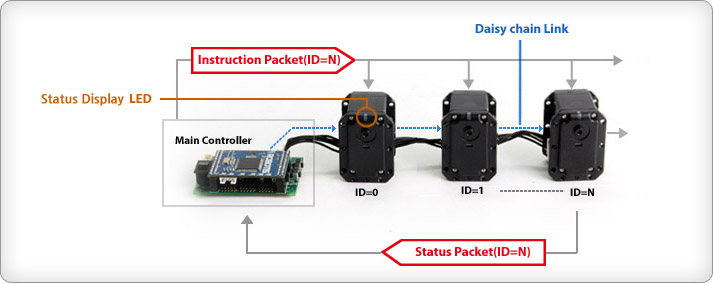
\includegraphics[width=8.5cm, height=4.5cm]{/dynamixel_daysi_chain.jpg}
		\caption{Servomotores dynamixel en conexión daisy chain.}
		\end{center}
	\end{figure}

	El sistema \textit{daisy chain} es un esquema de conecciones que forman una sucesión de enlaces, tal que el dispositivo A se encunetra conectado al sipositivo B y este, a su vez, se encuentra concectado a un dispositivo C y así sucesivamente. Es importante señalar que en este tipo de conección los dispositivos no forman redes, en tal caso el dispositivo C no podría estar conectado al dispositivo A. Otro aspecto importante de resaltar es que en este tipo de conecciones al no poder formar redes la comunicación se realiza dispositivo a dispositivo, por tanto los dispositivos ultimos en la cadena pueden presentar retraso o fallas electricas con respecto de los dispositivos primeros en orden de la cadena.\\  


%%%%%%%%%%%%%%%%%%%%%%%%%%%%%%%%%%%%%%%%%%%%%%%%%%%%%%%%%%
%%%%%%%%%%%%%%% DESCRIPCION DEL HARDWARE %%%%%%%%%%%%%%%%%
%%%%%%%%%%%%%%%%%%%%%%%%%%%%%%%%%%%%%%%%%%%%%%%%%%%%%%%%%%

	\section{Descripción de los elementos del sistema de manipulación}
		El sistema de Hardware del brazo robótico está compuesto por un total de 10 servomotores Dynamixel fabricados por la compañía Robotis \cite{dynamixelEpage}. Eta compañia cuenta con diversas gamas de modelos de servomotores según las necesidades de la apliación. A continuación se describirá el sistema en orden descendente.\\

		En la parte superior del brazo robótico se encuentran dos servomotores Dynamixel MX-106 conectados como maestro-esclavo, configurados en este modo trabajan de manera conjunta aumentando el par unitario de cada uno de los servomotores. Dadas las caracteristicas antes descritas en la tabla [] podemos observar que la configuración de servomotores entrega un par de torsión máximo a rotor bloqueado de $16.8N.m$ @ 12V. El sentido de giro positivo del arreglo de servomotores es el mostrado en la figura[4.8]. \\

		\begin{wrapfigure}{l}{0.60\textwidth}
			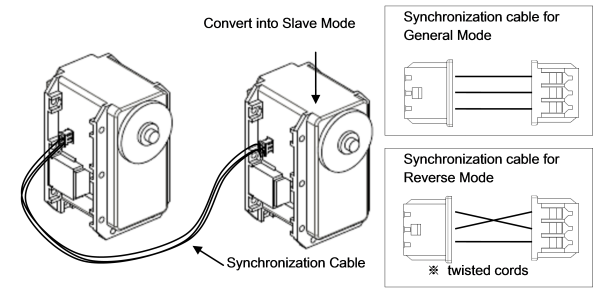
\includegraphics[width=8.0cm, height=4.5cm]{/mx106_MS.png}
			\caption{Configuración maestro-esclavo en servomotores dynamixel.}
		\end{wrapfigure}

		La configuración maestro-esclavo es un método de control simultaneo para dos servomotores Dynamixel, esta configuración es sumamente útil cuando se trata de construir una junta cuyo eje de acción es coincidente. Los motores respectivos maestro y esclavo deben estar conectados mediante un cable de sincronización. como se muestra en la figura[4.7]. El servomotor esclavo es directamente controlado por la señal PWM del maestro transmitida a travez del cable de sincronización. Es importante mencionar que la información de la posición, velocidad y corriente deseada es ignorada; puesto que esta información depende unicamente del maestro.\\  


		En la configuración maestro-esclavo el esclavo puede configurarse para adoptar un sentido de giro inverso en caso que el acoplamiento mecánico así lo requiera. Dentro de este modo el servomotor esclavo tendrá la misma velocidad que el motor maestro, solo diferenciado por el sentido inverso de giro.\\

		Posteriormente se encuentra un servomotor modelo MX-106, ubicado en una disposición horizontal. Unido a este servomotor se encuentra un eslabón obtenido mediante técnicas de manufactura aditiva. Dado que la construcción del brazo robótico esta pensanda desde el punto de vista antropomórfico  este conjunto de servomotores, el maestro-esclavo y el servomotor MX-106 describen los grados de libertad que emulan el movimiento de un hombro humano.\\

		\begin{wrapfigure}{r}{0.30\textwidth}
			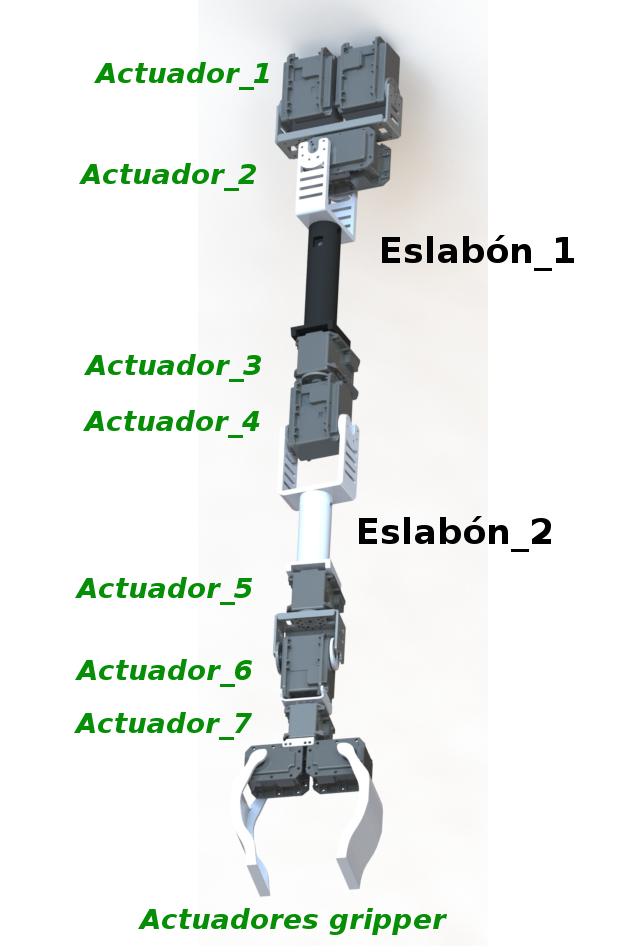
\includegraphics[width=4.5cm, height=12.5cm]{/brazo_4.jpg}
			\caption{Diseño asistido por computadora del brazo robótico del robot Justina.}
		\end{wrapfigure}

		El eslabón numero 1 obtenido mediante técnicas de manufactura aditiva funge como elemento de unión entre servomotores. Este elemento de unión cuenta con un peso total de **** Al final de este elemnto de unión se encuentra un servomotor MX-64 cuyo eje de acción es perpendicular respcto a la base el brazo. Directamente acoplado a este servomotor se encuentra otro servomotor modelo MX-106. Estos dos servomotores realizan el símil con un codo humano.\\

		Continuando en orden descendente, se encuentra un segundo eslabón utilizado como elemento de unión. En el extremo de este elemento se encuentra un servomotor MX-106, posteriormente un MX-64 y por último un servomoto modelo MX-28. Estos tres elementos construyen un sistema similar al de la muñeca de un brazo humano.\\

		Por último, se encuentra el efector final compuesto de dos actuadores MX-28 ubicados en disposición horizontal. En el eje de acción de cada uno de estos se encuentra una pieza obntenida de impresión 3D que funge como sujetador para manipular objetos.\\

		Como podemos observar el brazo robótico consta de un total de 10 servomotores conectados en \textit{daisy chain}. Dentro de este trabajo se realizó en analisis de la transmición de datos para cada uno de los servomotores. Para este analisis se partió de una configuración de conección previamente establecida, como se muestra en la figura []. Posteriormente se realizaron un total 1000 lecturas del registro \textit{Present Position} para cada uno de los actuadores. Se observó que la cantidad de datos perdidos era proporcional al número que el actuador tenía asignado en la cadena. De esta manera, se realizó la hipotesis que los datos se perdian a lo largo de la cadena de actuadores. Posteriormente se realizaron mediciones de voltaje a lo largo de la cadena, se observó una caida de 0.5V entre el actuador demominado A y los actuadores I-J.\\

		Los resultados obtenidos nos indicaron dos posibles ejes de acción. El primero de ellos, por facilidad de implementación, fue cambiar la velocidad de transmisión de datos para cada uno de los servomotores, yq ue una velocidad alta podría implicar una colision de datos en la transmisión, lo cúal conllevaría a el fenomeno que observamos. El segundo eje de acción fue el análisis del consumo de corrientes en cada uno de los actuadores. Este evento pudo haber ocasionado la caída de voltaje y posteriormente la perdida de datos al no estar adecuadamente alimentados los dispositivos.\\ 
		

		**** Cadena completa y muestra de las conexiones electricas (comparación antes y despues.)\\






	

%%%%%%%%%%%%%%%%%%%%%%%%%%%%%%%%%%%%%%%%%%%%%%%%%%%%%%%%%%%%%%%%
              %%%%%%  CINEMATICA DIRECTA   %%%%%%%%
%%%%%%%%%%%%%%%%%%%%%%%%%%%%%%%%%%%%%%%%%%%%%%%%%%%%%%%%%%%%%%%%

	\section{Cinemática directa}
		**** Teoría trasformaciones y medidas del brazo robotico
		**** Implementación (Descrpción con ROS)







%%%%%%%%%%%%%%%%%%%%%%%%%%%%%%%%%%%%%%%%%%%%%%%%%%%%%%%%%%%%%%%%
              %%%%%%  CINEMATICA INVERSA   %%%%%%%%
%%%%%%%%%%%%%%%%%%%%%%%%%%%%%%%%%%%%%%%%%%%%%%%%%%%%%%%%%%%%%%%%
	\section{Cinemática inversa}
